\documentclass[conference]{IEEEtran}
\IEEEoverridecommandlockouts
\usepackage{cite}
\usepackage{amsmath,amssymb}
\usepackage{graphicx}
\usepackage{booktabs}
\usepackage{multirow}
\usepackage{url}
\usepackage{xcolor}
\usepackage{tikz}
\usetikzlibrary{shapes.geometric,arrows.meta,positioning,fit,backgrounds}
\usepackage[capitalise]{cleveref}

\graphicspath{{figures/}}

\begin{document}

\title{Terrain-Dependent Effects of a Nomadic Aerial 5G Base Station on
Ground-Robot Command-and-Control: A Hardware-in-the-Loop Emulation Study}

\author{\IEEEauthorblockN{Innocent Nhlanhla Makhubela}
\IEEEauthorblockA{\textit{Search-and-Rescue Robotics and Nomadic 5G} \\
\texttt{makhubelainnocentnhlanhla@gmail.com}}}

\maketitle

\begin{abstract}
Aerial 5G base stations (gNBs) carried by unmanned aerial vehicles (UAVs) are a
promising way to deliver command-and-control (C2) and sensor backhaul to ground
robots in search-and-rescue (SAR) missions where fixed infrastructure is absent.
A natural question is whether the gNB should \emph{hover} over the search area or
\emph{roam} with the robots. We study this using a hardware-in-the-loop (HIL)
emulation that couples a real 5G stand-alone stack (OpenAirInterface gNB and user
equipment over the RF simulator, Open5GS core) to a physics simulator (Gazebo)
through an air-to-ground (A2G) channel bridge that applies per-link path loss,
terrain-specific non-line-of-sight (NLoS) excess, and log-normal shadowing in
real time; per-robot network namespaces force every C2 packet across the emulated
air interface. Across four terrains (open field, urban, forest, hills) each robot
runs a 6-hour trial split into a 3-hour \emph{static}-gNB phase and a 3-hour
\emph{nomadic}-gNB phase (continuous 3-D random walk). We find the effect of gNB
mobility on C2 availability is strongly \emph{terrain-dependent}: nomadism helps
a weak-link robot in line-of-sight (open field, $+32$ percentage points), is
neutral under localized building NLoS (urban), and is progressively harmful as
blockage becomes more pervasive (hills $-10.6$~pp, forest $-22$~pp). We further
show that maintaining C2 in NLoS at all requires a coverage controller that
reacts to \emph{measured} path loss rather than geometric distance, and that deep
outdoor-to-indoor penetration is effectively uncoverable at this link budget. We
release the emulation stack, the experiment automation, and the dataset.
\end{abstract}

\begin{IEEEkeywords}
UAV communications, 5G NR, aerial base station, air-to-ground channel,
search and rescue, hardware-in-the-loop emulation, OpenAirInterface, robot
command and control.
\end{IEEEkeywords}

\section{Introduction}
Search-and-rescue (SAR) operations increasingly deploy teams of ground robots to
explore hazardous areas, streaming video and sensor data back to operators while
receiving command-and-control (C2) updates such as waypoints and emergency stops.
In collapsed, remote, or disaster-struck environments, terrestrial cellular
infrastructure is frequently unavailable, motivating \emph{aerial} base stations:
a 5G New Radio (NR) gNB carried by an unmanned aerial vehicle (UAV) that provides
a nomadic radio cell over the search area~\cite{zeng2016wireless,mozaffari2019tutorial}.
Because the gNB is airborne and mobile, a mission planner faces a placement
decision that a fixed tower never poses: should the aerial gNB \emph{hover} at a
central vantage point, or \emph{roam} to follow the robots?

The answer is not obvious. A higher or repositioning aerial gNB can shorten the
air-to-ground (A2G) link and improve the line-of-sight (LoS) probability, which
argues for mobility~\cite{alhourani2014optimal}. But in cluttered environments the
same mobility can drive the gNB \emph{behind} obstacles relative to a robot, or
lengthen the propagation path through foliage, degrading the link. The trade-off
depends on the geometry \emph{and} on the physical mechanism of blockage --
buildings, trees, terrain, or building walls -- each of which loads the channel
differently.

Answering this question with fidelity is hard. Pure network simulators abstract
the protocol stack; pure robotics simulators abstract the radio. We instead build
a \emph{hardware-in-the-loop} (HIL) emulation that runs an unmodified 5G
stand-alone (SA) stack -- an OpenAirInterface (OAI) gNB and two user equipments
(UEs) over the RF simulator, with an Open5GS core -- and couples it to the Gazebo
physics simulator through a real-time A2G channel bridge. The bridge reads the
3-D poses of the UAV-gNB and the robots from the simulator and, every
0.5\,s, sets each link's attenuation in the RF simulator from an A2G
path-loss model plus a terrain-specific NLoS term and correlated shadow fading.
Crucially, we place each UE's tunnel interface in its own Linux network namespace
so that C2 traffic (base~$\rightarrow$~robot) genuinely traverses the emulated air
interface in both directions rather than short-circuiting over the host loopback.
The result is an honest, protocol-complete measurement of C2 availability,
throughput, latency, and radio-link stability as a function of gNB and robot
motion in a chosen terrain.

\noindent\textbf{Contributions.}
\begin{itemize}
  \item A reproducible HIL emulation coupling a full OAI/Open5GS 5G~SA stack to
  Gazebo through a real-time A2G channel bridge, with namespace isolation that
  makes the downlink C2 path physically honest (\cref{sec:system}).
  \item A terrain-parameterized A2G channel model that shares a single obstacle
  geometry between the physics world and the radio channel for urban buildings,
  forest foliage, knife-edge terrain, and 3GPP outdoor-to-indoor (O2I)
  penetration (\cref{sec:channel}).
  \item An NLoS-aware coverage controller that keeps robots connected by reacting
  to \emph{measured} path loss, without which cluttered terrains suffer an
  unrecoverable radio-link-failure (RLF) cascade (\cref{sec:controller}).
  \item A controlled static-vs-nomadic gNB study over four terrains and 6~hours
  each, establishing that the sign of the mobility effect flips with the
  pervasiveness of blockage, and characterizing the O2I coverage limit
  (\cref{sec:results}).
\end{itemize}

\section{Related Work}
\label{sec:related}
\textbf{UAV-assisted communications.} The use of UAVs as flying base stations or
relays is surveyed in~\cite{zeng2016wireless,mozaffari2019tutorial}. A central
result is the existence of an optimal altitude that balances free-space loss
against LoS probability for a low-altitude platform~\cite{alhourani2014optimal}.
Most of this literature optimizes \emph{placement} analytically or in
system-level simulation under statistical channel models; comparatively little
work evaluates a \emph{running} 5G stack driving \emph{physical} robot mobility,
which is our focus.

\textbf{A2G channel models.} The elevation-angle-dependent LoS probability
and excess-loss formulation of~\cite{alhourani2014optimal} and the 3GPP channel
models~\cite{3gpp38901,3gpp36777} underpin our path-loss core. For terrain-specific
excess we use the Weissberger vegetation model~\cite{weissberger1982} for foliage
and knife-edge diffraction~\cite{ituP526} for hills, and the 3GPP O2I penetration
term~\cite{3gpp38901} for indoor.

\textbf{Emulation platforms.} OpenAirInterface provides an open, standard-compliant
5G stack with an RF simulator that replaces radios with a TCP channel, enabling
software-only experiments~\cite{nikaein2014oai}. Open5GS supplies the 5G core.
Namespace- and container-based network emulation in the style of
Mininet~\cite{lantz2010mininet} lets us isolate each UE's data path. Gazebo
provides rigid-body physics and sensor simulation for the
robots~\cite{koenig2004gazebo}. Our contribution is not any one component but
their real-time coupling through a geometry-consistent A2G channel, and the
namespace design that makes the C2 downlink honest.

\textbf{Robot connectivity and SAR.} Connectivity-aware planning keeps robots
within coverage of a base or relay. We instead ask the dual question -- how a
mobile base should behave given roaming robots -- and measure it end-to-end on a
real stack rather than under an abstract link model.

\section{System Architecture}
\label{sec:system}
\Cref{fig:arch} shows the emulation. Three subsystems run concurrently on one
host and are joined by the channel bridge.

\begin{figure}[t]
\centering
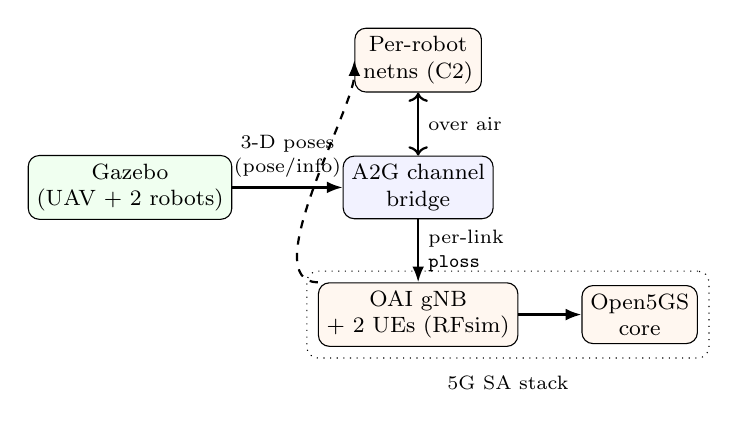
\begin{tikzpicture}[
  font=\footnotesize,
  box/.style={draw, rounded corners, align=center, minimum height=7mm,
              inner sep=3pt, fill=blue!5},
  sim/.style={box, fill=green!6},
  net/.style={box, fill=orange!6},
  arr/.style={-{Latex[length=2mm]}, thick},
  node distance=5mm and 8mm]
  \node[sim] (gz) {Gazebo\\ (UAV + 2 robots)};
  \node[box, right=14mm of gz] (br) {A2G channel\\ bridge};
  \node[net, below=8mm of br] (oai) {OAI gNB\\ + 2 UEs (RFsim)};
  \node[net, right=8mm of oai] (core) {Open5GS\\ core};
  \node[net, above=8mm of br, xshift=0mm] (ns) {Per-robot\\ netns (C2)};
  \draw[arr] (gz.east) -- node[above,align=center]{\scriptsize 3-D poses\\[-1pt]\scriptsize (pose/info)} (br.west);
  \draw[arr] (br.south) -- node[right,align=left]{\scriptsize per-link\\[-1pt]\scriptsize \texttt{ploss}}(oai.north);
  \draw[arr] (oai.east) -- (core.west);
  \draw[arr,<->] (ns.south) -- node[right]{\scriptsize over air}(br.north);
  \draw[arr,dashed] (oai.north west) .. controls +(left:8mm) and +(down:6mm) .. (ns.west);
  \begin{scope}[on background layer]
    \node[draw, dotted, rounded corners, fit=(oai)(core), inner sep=4pt,
          label={[yshift=-1mm]below:\scriptsize 5G SA stack}] {};
  \end{scope}
\end{tikzpicture}
\caption{HIL emulation. Gazebo streams UAV/robot poses to the channel bridge,
which sets each RF-simulator link's attenuation in real time. UE tunnel
interfaces live in per-robot network namespaces so the C2 downlink crosses the
air interface honestly.}
\label{fig:arch}
\end{figure}

\textbf{5G stack.} An OAI gNB and two OAI UEs run over the RF simulator on 5G~NR
band~n78 (3.32\,GHz, 40\,MHz, numerology~1), attached to
an Open5GS 5G core. The RF simulator exposes a telnet control interface through
which the per-link channel attenuation can be set at run time.

\textbf{Physics.} Gazebo simulates one UAV (the aerial gNB) and two differential-drive
ground robots, publishing all 3-D poses on a pose topic. Robots are driven by
velocity commands with pose feedback, so motion is kinematic rather than
teleported.

\textbf{Channel bridge.} A Python process subscribes to the pose topic and, at
2\,Hz, computes each link's attenuation (\cref{sec:channel}) and writes
it to the RF simulator over telnet as a positive path-loss magnitude. The same
obstacle geometry that Gazebo renders is imported by the bridge, so the radio
channel and the visible world are consistent by construction.

\textbf{Namespace isolation.} Without isolation, both UE IP addresses are local to
the host, so downlink traffic to a robot (C2 commands, TCP ACKs) is delivered over
loopback and never touches the radio. We move each UE's tunnel device into its own
network namespace; the UE process keeps its open file descriptor across the move,
so the stack is untouched but base-to-robot traffic now genuinely traverses core,
gNB, and the emulated air interface. This makes the C2 metric an honest
measurement.

\section{Air-to-Ground Channel Model}
\label{sec:channel}
For a robot at horizontal distance $d$ from the UAV nadir and UAV height $h$, the
3-D distance is $r=\sqrt{d^2+(h-h_u)^2}$ with UE height $h_u$. The core path loss
combines free-space loss with an elevation-angle-dependent LoS/NLoS
mixture~\cite{alhourani2014optimal}:
\begin{align}
\mathrm{FSPL} &= 20\log_{10} r + 20\log_{10} f - 147.55, \\
p_{\mathrm{LoS}} &= \frac{1}{1 + a\,e^{-b(\theta - a)}},\quad
\theta = \arctan\!\frac{h-h_u}{d}, \\
\mathrm{PL} &= \mathrm{FSPL} + p_{\mathrm{LoS}}\eta_{\mathrm{LoS}}
              + (1-p_{\mathrm{LoS}})\eta_{\mathrm{NLoS}},
\end{align}
where $f$ is the carrier frequency and $(a,b,\eta_{\mathrm{LoS}},
\eta_{\mathrm{NLoS}})$ are environment constants. The bridge reports the delta of
$\mathrm{PL}$ relative to a fixed reference distance, adds a per-link baseline that
calibrates the RF-simulator operating point, and clamps the total to the model
range.

\textbf{Terrain-specific NLoS excess.} Each world contributes an additive term
$\Delta_{\mathrm{env}}$ evaluated on the \emph{shared} geometry:
\begin{itemize}
  \item \emph{Urban:} building footprints; if the UAV$\to$robot segment
  intersects a building, a hard NLoS excess applies (LoS is otherwise clear).
  \item \emph{Forest:} $\Delta_{\mathrm{env}}$ grows with the foliage path length
  through tree canopies (Weissberger form~\cite{weissberger1982}).
  \item \emph{Hills:} knife-edge diffraction loss over terrain
  ridges~\cite{ituP526}.
  \item \emph{Indoor:} a 3GPP O2I penetration term (fixed wall loss plus a
  per-metre depth loss) whenever the robot is inside the building
  footprint~\cite{3gpp38901}.
\end{itemize}

\textbf{Shadow fading.} On top of the smoothed mean we add correlated log-normal
shadowing (larger variance under NLoS), decorrelated over distance moved so that a
stationary robot holds a steady shadow offset and only motion mixes in new fading.

\section{NLoS-Aware Coverage Controller}
\label{sec:controller}
A naive coverage rule keeps each robot within a geometric \emph{safe radius}
computed from the open-field model at the current UAV altitude. We found this
fails badly in every NLoS terrain: a robot can sit well inside the safe radius yet
be blocked (path loss near the RLF cliff), because the distance rule is blind to
buildings, trees, and terrain. When such a robot loses the link, an RLF is
declared; and because a UE cannot complete cell (re)synchronization while buried
in deep NLoS, the recovery -- restarting the UE softmodem -- \emph{fails to
re-attach} (``tunnel never reappeared''). The controller then retries
indefinitely, and the robot stays dark. In a first full run this produced $86$
failed re-attachments in the urban world and near-zero availability for the weak
robot.

We therefore make the controller react to the \emph{measured} path loss $p$ (read
cheaply from the bridge log tail at driver rate), not to distance:
\begin{itemize}
  \item \emph{Soft:} if $p$ is elevated, steer the robot \emph{toward} the gNB
  ground track (raising the elevation angle and reducing NLoS depth), with
  reactive obstacle avoidance still routing around walls.
  \item \emph{Hard:} if $p$ stays near the cliff, teleport the robot to a small
  radius from the gNB (a steep elevation angle gives near-certain LoS in every
  world) \emph{before} it dies, since a re-attach cannot rescue a UE with no
  signal.
\end{itemize}
For the indoor mission, where the robot \emph{must} occupy the building, pulling
it toward the gNB would defeat the task; instead a robot whose $p$ nears the cliff
\emph{retreats along its reversed entry path toward the door}, where O2I loss
falls and the UE survives, then re-enters. This prevention-first design converts
the unrecoverable cascade into rare, short, recoverable outages
(\cref{sec:results}).

\section{Experimental Methodology}
\label{sec:method}
\textbf{Worlds.} Open field (LoS baseline), urban (building NLoS), forest
(foliage), hills (diffraction), and indoor (O2I). All share the identical robot,
UAV, and radio configuration; only the world geometry and its channel term differ.

\textbf{Protocol.} Each world runs a single 6-hour trial in two phases. In
\emph{phase~1} ($0$--3\,h) the gNB hovers statically. In \emph{phase~2}
(3--6\,h) the gNB performs a continuous 3-D random walk over a
bounded box (never dwelling). Both ground robots free-patrol throughout, so the
only variable between phases is gNB mobility. \Cref{fig:traj} contrasts the two
regimes.

\textbf{Metrics.} Every $\sim$15--60\,s we log, per robot: C2 round-trip loss and
latency (ICMP base$\to$robot over the air), served TCP and fixed-rate UDP uplink
throughput (modelling a sensor/video feed), UDP loss and jitter, and the modem's
SS-RSRP, SS-SINR, and downlink BLER, together with the current path loss and the
gNB--robot slant distance. We define \emph{C2 availability} as the fraction of
samples with less than 100\% C2 loss. A background watchdog logs every RLF
recovery and every controller intervention.

\textbf{Data hygiene.} A single physical stack must serve only one trial: two
concurrent trials share the same robots and gNB and silently corrupt each other,
which we guard against with an exclusive campaign lock. Runs that predate the
NLoS-aware controller, or that suffered the re-attach cascade, are excluded; the
four reported worlds are clean 6-hour trials ($733$, $721$, $482$, and $974$
samples for open field, urban, forest, and hills respectively).

\begin{figure}[t]
\centering
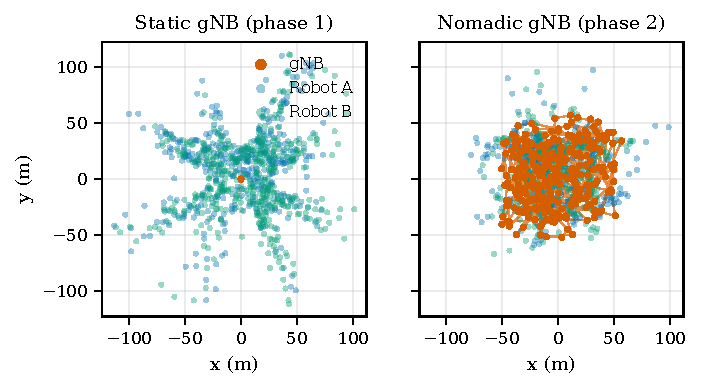
\includegraphics[width=\columnwidth]{fig_gnb_traj.pdf}
\caption{Top-down gNB and robot positions in the urban world. In phase~1 (left)
the gNB is fixed at the origin and robots roam widely; in phase~2 (right) the gNB
random-walks and the coverage controller keeps robots clustered around its live
ground track.}
\label{fig:traj}
\end{figure}

\section{Results}
\label{sec:results}

\subsection{C2 availability: the mobility effect flips with terrain}
\Cref{fig:c2} and \cref{tab:main} give the headline. In \emph{open field}, gNB
mobility \emph{helps}: the weak-link robot's C2 availability rises from $56.5\%$
(static) to $88.7\%$ (nomadic), a $+32$~pp gain, because the wandering gNB
periodically drifts closer and rescues a robot stranded near the coverage edge
(its mean distance falls from $91$ to $75$\,m). The strong robot is already near
$98\%$ in both phases. In \emph{urban}, mobility is \emph{neutral}
($\sim$$96$--$98\%$ in both phases): localized buildings leave LoS pockets, and the
controller keeps robots in them regardless of gNB motion. In \emph{hills} and
\emph{forest}, mobility \emph{hurts}, and the magnitude tracks how pervasive the
blockage is: knife-edge terrain costs $-10.6$~pp (robot-averaged) while
everywhere-present foliage costs $-22$~pp, collapsing both robots to
$\sim$$73$--$75\%$. \Cref{fig:delta} summarizes the per-robot deltas.

\begin{table}[t]
\centering
\caption{C2 availability and mean link metrics by world and gNB phase
(robot-averaged unless noted). $\Delta$ is nomadic$-$static C2.}
\label{tab:main}
\footnotesize
\begin{tabular}{@{}llrrrr@{}}
\toprule
World & Phase & C2 (\%) & PLoss & SINR & TCP \\
      &       &         & (dB)  & (dB) & (Mb/s) \\
\midrule
\multirow{2}{*}{Open field}
 & Static  & 76.8 & 16.5 & 35.1 & 9.7  \\
 & Nomadic & 93.5 & 14.2 & 38.8 & 13.1 \\
\cmidrule(l){2-6}
 & \multicolumn{1}{r}{$\Delta$} & \textbf{+16.7} & & & \\
\midrule
\multirow{2}{*}{Urban}
 & Static  & 97.0 & 8.8  & 43.8 & 17.6 \\
 & Nomadic & 96.9 & 10.4 & 42.6 & 16.1 \\
\cmidrule(l){2-6}
 & \multicolumn{1}{r}{$\Delta$} & \textbf{$-$0.1} & & & \\
\midrule
\multirow{2}{*}{Hills}
 & Static  & 98.9 & 3.9  & 45.7 & 21.6 \\
 & Nomadic & 88.3 & 9.3  & 44.2 & 19.4 \\
\cmidrule(l){2-6}
 & \multicolumn{1}{r}{$\Delta$} & \textbf{$-$10.6} & & & \\
\midrule
\multirow{2}{*}{Forest}
 & Static  & 96.2 & 10.8 & 40.9 & 15.1 \\
 & Nomadic & 74.2 & 21.7 & 32.5 & 3.2  \\
\cmidrule(l){2-6}
 & \multicolumn{1}{r}{$\Delta$} & \textbf{$-$22.0} & & & \\
\bottomrule
\end{tabular}
\end{table}

\begin{figure}[t]
\centering
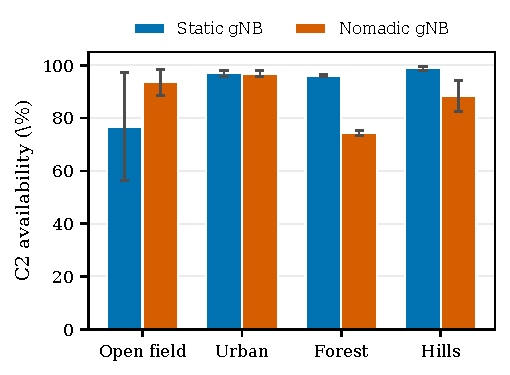
\includegraphics[width=\columnwidth]{fig_c2_avail.pdf}
\caption{C2 availability by world and gNB phase (bar = robot mean; whiskers span
the two robots). Nomadism helps in open field, is neutral in urban, and hurts in
hills and forest.}
\label{fig:c2}
\end{figure}

\begin{figure}[t]
\centering
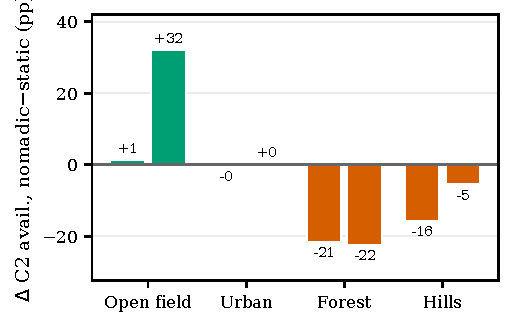
\includegraphics[width=\columnwidth]{fig_nomadic_effect.pdf}
\caption{Per-robot change in C2 availability from static to nomadic gNB. The
weak-link robot in open field gains most; both robots lose most in forest.}
\label{fig:delta}
\end{figure}

\subsection{Path loss and throughput explain the effect}
\Cref{fig:ploss} bins measured path loss against gNB--robot slant distance per
world. Open field and hills sit low (steep LoS-dominated curves); forest rises
sharply because a longer slant path cuts through more canopy; urban is
intermediate with building-driven jumps. Mobility moves robots along these curves:
in forest, nomadism raises mean path loss from $\sim$11 to $\sim$22\,dB and drives
served TCP throughput from $15.1$ to $3.2$\,Mb/s while fixed-rate UDP loss climbs
above $70\%$ (\cref{fig:tput}). In urban and open field, throughput is essentially
preserved or improved. \Cref{fig:sinr} shows the SS-SINR distributions: all worlds
are healthy in the LoS-dominated regime, but forest develops a heavy low-SINR tail
under nomadism.

\begin{figure}[t]
\centering
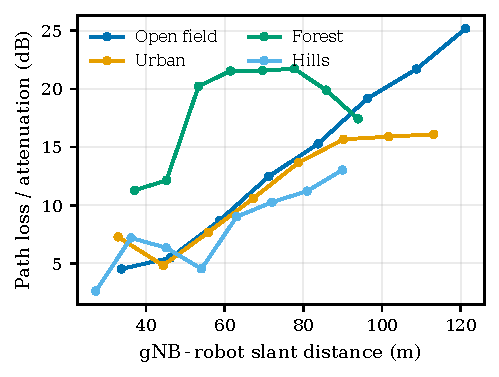
\includegraphics[width=\columnwidth]{fig_ploss_dist.pdf}
\caption{Measured path loss vs.\ gNB--robot slant distance (binned means). Forest
rises steeply with distance (foliage path length); hills and open field stay low.}
\label{fig:ploss}
\end{figure}

\begin{figure}[t]
\centering
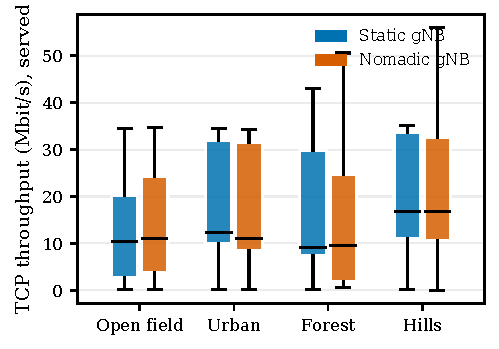
\includegraphics[width=\columnwidth]{fig_throughput.pdf}
\caption{Served TCP throughput by world and phase. Forest collapses under a
nomadic gNB; urban and open field are preserved.}
\label{fig:tput}
\end{figure}

\begin{figure}[t]
\centering
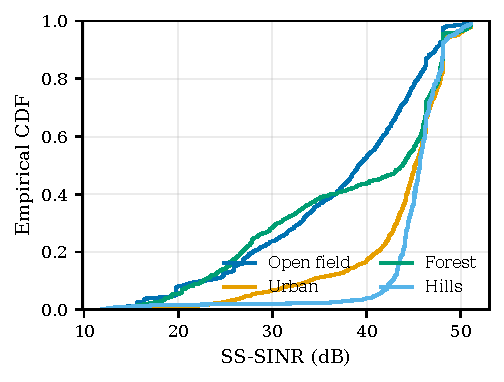
\includegraphics[width=\columnwidth]{fig_sinr_cdf.pdf}
\caption{Empirical CDF of SS-SINR. Forest develops a heavy low-SINR tail;
other worlds remain in the high-SINR regime.}
\label{fig:sinr}
\end{figure}

\subsection{Link recovery: prevention beats reaction}
\Cref{fig:events} counts link events per 6-hour run. With the NLoS-aware
controller, the re-attach cascade is eliminated in urban and hills (zero failed
re-attaches) and contained in forest ($16$), where the controller intervenes
$574$ times -- roughly once every $37$\,s -- to keep robots out of foliage dead
zones. The cost of prevention is visible in \cref{fig:traj}: the controller keeps
NLoS robots closer to the gNB than free roaming would, so their trajectories are
more gNB-centred. This is the price of any valid measurement in NLoS: without it,
the terrains do not merely degrade, they fail to produce data.

\begin{figure}[t]
\centering
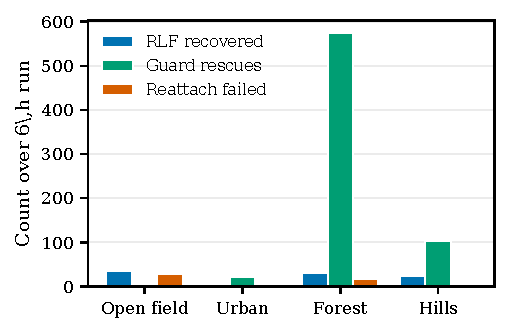
\includegraphics[width=\columnwidth]{fig_events.pdf}
\caption{Link events over each 6-hour run. Forest requires by far the most
controller interventions; urban and hills incur zero failed re-attaches.}
\label{fig:events}
\end{figure}

\subsection{Indoor: a coverage limit, not a tuning problem}
The outdoor-to-indoor world is qualitatively different. The fixed wall-penetration
term plus the link baseline places the \emph{entire} building interior near the
RLF cliff -- depth barely matters -- so shadow spikes trip RLF repeatedly, and each
$\sim$2-minute re-attach dominates the timeline. Lowering the gNB to hover
directly overhead (cutting $\sim$7\,dB of A2G loss) and adding the retreat-to-door
recovery removes the cascade and keeps robots alive, but C2 availability remains
only $12$--$18\%$ (\cref{fig:indoor}). We interpret this as a genuine finding
rather than a defect: a ground robot cannot hold C2 deep inside a building at this
link budget, and \emph{leaving the building is the only recovery} -- exactly the
behaviour the retreat controller encodes.

\begin{figure}[t]
\centering
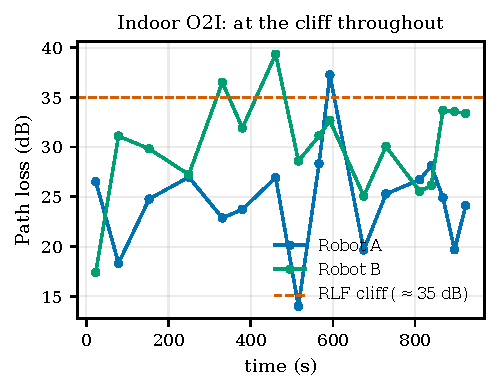
\includegraphics[width=\columnwidth]{fig_indoor.pdf}
\caption{Indoor O2I path loss over time (low-hovering gNB). Both robots sit at the
RLF cliff throughout; the interior offers no reliably covered pocket.}
\label{fig:indoor}
\end{figure}

\section{Discussion}
\label{sec:discussion}
The unifying explanation is that gNB mobility changes the \emph{propagation path},
and whether that helps depends on how blockage is distributed. In LoS, a moving
gNB is pure geometric benefit: it can shorten links and rescue edge robots, so
nomadism helps the weak robot most. Where blockage is \emph{localized} (urban
buildings), a controller can keep robots in LoS pockets and mobility washes out.
Where blockage is \emph{pervasive} (forest canopy), there is no pocket to hold:
any repositioning that lengthens the ground path lengthens the foliage path, so
mobility is strictly harmful, and the damage scales with blockage density
(hills~$<$~forest). For SAR planning this suggests a simple heuristic: \emph{hover}
a nomadic gNB when the environment is cluttered and pervasive, and \emph{roam} it
only when links are LoS-dominated or robots risk stranding at the coverage edge.

\section{Threats to Validity}
\label{sec:threats}
\textbf{Emulated channel.} Attenuation is applied by the RF simulator from our A2G
model; absolute values depend on model constants and the simulator's noise floor,
so we emphasize \emph{relative} static-vs-nomadic effects within a fixed
calibration rather than absolute link budgets. \textbf{Controller coupling.} The
coverage controller is necessary to obtain data in NLoS but alters robot
trajectories (more gNB-centred), so the reported effects are conditional on
prevention-based coverage keeping; free-roaming robots would simply lose the link.
\textbf{Single cell, two UEs.} We study one gNB and two robots; multi-cell
handover and many-robot contention are future work. \textbf{Sampling rate.} Under
outage the expensive per-sample probes time out, so heavily degraded phases yield
fewer samples (e.g.\ forest phase~2); fine-grained path loss is nonetheless logged
continuously by the bridge. \textbf{Indoor calibration.} The O2I result reflects
one building geometry and link budget; a different penetration term or baseline
would move the coverage limit, though not the qualitative conclusion that deep O2I
is the hardest case.

\section{Conclusion}
\label{sec:conclusion}
We built a hardware-in-the-loop emulation that runs a complete 5G~SA stack against
physics-simulated robot and UAV motion through a geometry-consistent air-to-ground
channel, with namespace isolation that makes the command-and-control downlink
physically honest. Using it to compare a static and a nomadic aerial gNB across
four terrains for six hours each, we showed that the effect of gNB mobility on C2
availability is terrain-dependent and changes sign with the pervasiveness of
blockage: helpful in line-of-sight (open field, $+32$~pp for the weak robot),
neutral under localized urban NLoS, and increasingly harmful under diffraction and
foliage (hills $-10.6$, forest $-22$~pp). We further showed that maintaining
connectivity in NLoS at all requires a coverage controller that reacts to measured
path loss rather than geometric distance, and that deep outdoor-to-indoor
penetration is effectively uncoverable at this link budget, with retreat-to-door
as the only recovery. The emulation stack, experiment automation, and dataset are
released to support reproduction and extension to multi-cell, many-robot SAR
scenarios.

\begin{thebibliography}{00}
\bibitem{zeng2016wireless} Y.~Zeng, R.~Zhang, and T.~J.~Lim, ``Wireless
communications with unmanned aerial vehicles: opportunities and challenges,''
\emph{IEEE Commun. Mag.}, vol.~54, no.~5, pp.~36--42, 2016.
\bibitem{mozaffari2019tutorial} M.~Mozaffari, W.~Saad, M.~Bennis, Y.-H.~Nam, and
M.~Debbah, ``A tutorial on UAVs for wireless networks: applications, challenges,
and open problems,'' \emph{IEEE Commun. Surveys Tuts.}, vol.~21, no.~3,
pp.~2334--2360, 2019.
\bibitem{alhourani2014optimal} A.~Al-Hourani, S.~Kandeepan, and S.~Lardner,
``Optimal LAP altitude for maximum coverage,'' \emph{IEEE Wireless Commun. Lett.},
vol.~3, no.~6, pp.~569--572, 2014.
\bibitem{3gpp38901} 3GPP, ``Study on channel model for frequencies from 0.5 to
100 GHz,'' TR~38.901, 2020.
\bibitem{3gpp36777} 3GPP, ``Study on enhanced LTE support for aerial vehicles,''
TR~36.777, 2017.
\bibitem{weissberger1982} M.~A.~Weissberger, ``An initial critical summary of
models for predicting the attenuation of radio waves by trees,'' ECAC-TR-81-101,
1982.
\bibitem{ituP526} ITU-R, ``Propagation by diffraction,'' Recommendation P.526.
\bibitem{nikaein2014oai} N.~Nikaein \emph{et al.}, ``OpenAirInterface: a flexible
platform for 5G research,'' \emph{ACM SIGCOMM Comput. Commun. Rev.}, vol.~44,
no.~5, pp.~33--38, 2014.
\bibitem{lantz2010mininet} B.~Lantz, B.~Heller, and N.~McKeown, ``A network in a
laptop: rapid prototyping for software-defined networks,'' in \emph{Proc. ACM
SIGCOMM HotNets}, 2010.
\bibitem{koenig2004gazebo} N.~Koenig and A.~Howard, ``Design and use paradigms for
Gazebo, an open-source multi-robot simulator,'' in \emph{Proc. IEEE/RSJ IROS},
2004, pp.~2149--2154.
\end{thebibliography}

\end{document}
